La luce di scintillazione prodotta in un mezzo dal passaggio di una radiazione può essere raccolta da opportuni fotosensori, per produrre un segnale elettrico e dare informazioni sulla radiazione originaria. I fotosensori che devono essere accoppiati a uno scintillatore devono essere estremamente sensibili, quindi in grado di produrre un segnale elettrico anche quando vengono colpiti da pochi fotoni. Addirittura certe volte si parla di rivelatori a singolo fotone, quindi anche il singolo fotone può dar luogo a un segnale elettrico rivelabile. In questo capitolo andremo a vedere diverse tipologie di fotosensori, quali i fotomoltiplicatori ma anche rivelatori di più recente produzione come i diodi a valanga e i fotomoltiplicatori realizzati in silicio.

\section{Fotomoltiplicatori}

La prima tipologia di fotosensori che studieremo sono i fotomoltiplicatori.

\subsection{Schema di funzionamento}

Osserviamo come funzione un moltiplicatore:

\begin{figure}[H]
   \centering
   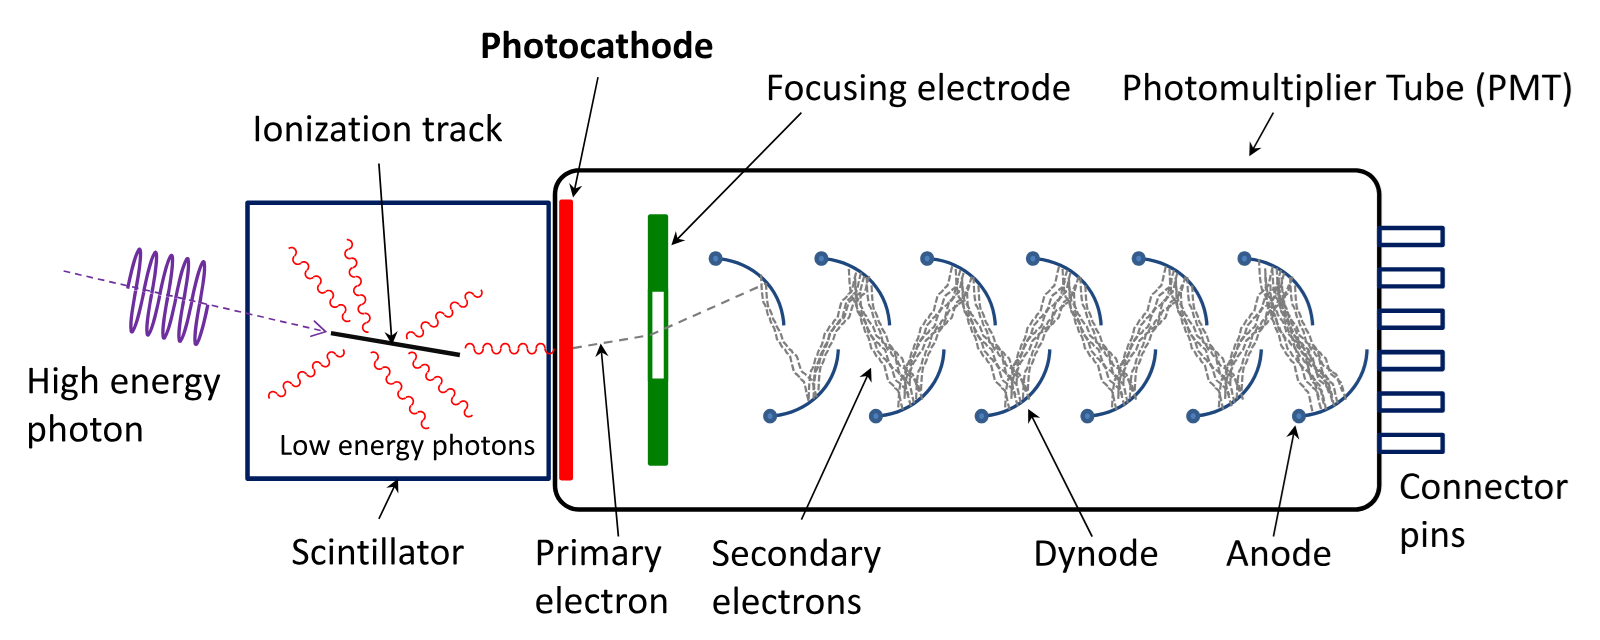
\includegraphics[width=0.8\textwidth]{immagini/fotomoltiplicatore.png}
\end{figure}

Quando arriva una radiazione che interagisce con lo scintillatore in un punto, viene emessa della luce e i fotoni, o attraverso delle riflessioni multiple o perché vengono emessi con la direzione giusta, arrivano alla finestra di ingresso del fotomoltiplicatore che prende il nome di fotocatodo, il quale non è altro che una superficie tipicamente vetrosa che viene rivestita di un materiale con un basso potenziale di estrazione in cui quindi può facilmente avvenire effetto fotoelettrico. In questo modo, un fotone che incide darà luogo ad effetto fotoelettrico e verrà quindi emesso un elettrone. Quest'ultimo viene guidato verso una zona dove sono presenti degli elettrodi che prendono il nome di dinodi. \E chiaro che l'elettrone viene guidato attraverso un campo elettrico, quindi questi dinodi vengono posizionati ad un potenziale via via crescente, cioè ogni dinodo ha un potenziale maggiore rispetto al precedente, in maniera tale che gli elettroni vengono guidati attraverso questa catena di dinodi.

L'elettrone che viene generato per effetto fotoelettrico, non appena incide sul primo dinodo, permette l'emissione di un certo numero di elettroni, in quanto viene ceduta dell'energia che serve ad estrarre altri elettroni dal primo dinodo; a questo punto questi elettroni vengono accelerati verso il secondo dinodo e ognuno di questi elettroni daà luogo, allo stesso modo, ad altri elettroni. Parliamo quindi di meccanismo di moltiplicazione, in quanto per ogni dinodo un elettrone incidente può estrarre un certo numero di elettroni.

Tale processo avviene lungo tutta la struttura, quindi man mano il numero di elettroni emessi che viaggia attraverso la catena di dinodi aumenta attraverso una legge di potenza fino a quando arriva all'ultimo dinodo, che non è altro che l'anodo, da cui viene poi prelevato il segnale il quale è un segnale in carica, cioè una corrente, per cui si adopera una resistenza in modo da produrre una un segnale in tensione che è quello che poi adoperiamo e possiamo visualizzare all'oscilloscopio. Si tratta quindi di un segnale che in linea di principio dovrebbe essere proporzionale al numero di elettroni che sono stati generati da questo fotomoltiplicatore e questo numero di elettroni dipende da quanti fotoni hanno inciso sul fotomoltiplicatore, quindi da quanti fotoni sono stati prodotti durante il processo di scintillazione. Si tratta dunque di una catena che permette di mantenere una certa proporzionalità e quindi di avere in uscita un segnale che dà indicazioni sull'energia depositata all'interno dello scintillatore.

A causa di tale schema di funzionamento, il fotomoltiplicatore è un oggetto abbastanza esteso, in quanto dobbiamo avere uno schema di dinodi che presenta delle geometrie particolari tali da poter guidare gli elettroni attraverso i dinodi ed inoltre questi devono avere delle forme caratteristiche. Ecco perché si chiama fotomoltiplicatore, perché non solo è un rivelatore di fotoni ma in più è un moltiplicatore, quindi da un singolo elettrone che corrisponde alla rivelazione di un fotone si produce una cascata di elettroni verso l'anodo con un certo fattore di moltiplicazione.

\subsection{Fotocatodo}
Guardiamo un po' più nel dettaglio i diversi componenti del fotomoltiplicatore, partendo dal fotocatodo.

Il fotocatodo rappresenta sostanzialmente la finestra di ingresso al fotomoltiplicatore, quindi è la zona dove devono incidere i fotoni di scintillazione. Normalmente è realizzato su un materiale vetroso\footnote{Il motivo è che così si assicura un indice di rifrazione simile a quello dello scintillatore o delle eventuali guide di luce che si utilizzano per accoppiare lo scintillatore col fotosensore, in maniera tale da evitare fenomeni di rifrazione.} che viene rivestito di un materiale caratterizzato da un un basso lavoro di estrazione. Normalmente vengono utilizzati dei materiali semi-conduttori per il semplice fatto che gli elettroni che vengono emessi per effetto fotoelettrico riescono più facilmente a lasciare il fotocatodo e a fuoriuscire. Come sappiamo, l'energia cinetica con cui l'elettrone fuoriesce dipende dall'energia del fotone incidente e dal potenziale di estrazione, essendo data dalla differenza tra queste: poiché i fotoni di scintillazione, ricadendo nell'ultravioletto, hanno energie di circa 3 eV, mentre i materiali che si adoperano hanno un potenziale di circa $1.5-2$ eV, l'elettrone che viene emesso ha un'energia abbastanza bassa, di pochi elettronVolt.

Bisogna inoltre ricordare che, essendo un materiale con così basso lavoro di estrazione, potrebbe verificarsi anche un'emissione spontanea per effetto termico. Ad esempio a temperatura ambiente gli elettroni hanno un'energia media di $0,025$ eV, quindi alcuni elettroni potrebbero effettivamente essere emessi per effetto termico. Siccome noi non avvertiamo alcuna differenza tra l'elettrone che viene emesso perché ha inciso un fotone o l'elettrone che viene messo per effetto termico in quanto entrambi daranno luogo a tutti i processi che abbiamo appena visto, ciò rappresenta un problema perché rappresentano una fonte di rumore che si va a sommare al reale segnale fisico dovuto alla rivelazione di fotoni di scintillazione. Una soluzione banale a tale problema è quella di operare a temperature più basse per ridurre la probabilità di emissione di elettroni per effetto termico.

Come abbiamo detto, l'effetto termico non è del tutto trascurabile. Infatti a temperatura ambiente gli elettroni hanno un'energia media di $0.025$ eV, dunque una certa frazione di elettroni può avere un'energia superiore a questo valore di energia media che risulta sufficiente quindi per poter sfuggire dal materiale. In generale, a temperatura ambiente la frequenza di emissione, cioè il numero di elettroni che vengono emessi al secondo, nei metalli corrisponde a circa 100 elettroni al secondo per ogni metro quadro mentre nei materiali semi-conduttori arriva fino a $10^6-10^8$ elettroni al secondo per metro quadro. Capiamo quindi che tale processo non è per niente trascurabile e l'effetto di questa emissione provoca quindi una corrente di elettroni che prende il nome di dark current, perché è una corrente che è sempre presente anche quando non incide luce sul fotosensore, quindi in condizioni di oscurità e purtroppo questo è uno dei parametri di cui si deve tener conto in un fotomoltiplicatore perché rappresenta qualcosa che si insomma al segnale.

Un altro aspetto che si deve tenere in conto quando si sceglie il fotocatodo riguarda l'efficienza di rivelazione. Finora infatti abbiamo schematizzato il processo dicendo che la radiazione incide e produce effetto fotoelettrico, ma in realtà la probabilità con cui avviene questo effetto dipende dalla lunghezza d'onda della radiazione incidente. Possiamo quindi andare a definire, in base al tipo di materiale adoperato, quanto vale la quantum efficiency cioè l'efficienza quantica, che rappresenta il numero di fotoelettroni emessi sul numero di fotoni incidenti:
\begin{equation*}
   \text{Quantum Efficiency }(QE)
   =\frac{\text{n° fotoelettroni emessi}}{\text{n° fotoni incidenti}}
\end{equation*}
Per fare un esempio, se incidessero 100 fotoni di scintillazione e in corrispondenza ad ogni fotone di scintillazione otteniamo un elettrone o fotoelettrone, allora l'efficienza sarebbe al 100\%. \E chiaro che nella realtà non abbiamo efficienze così elevate: tipicamente ci aggiriamo intorno al 20-30\%, quindi in media $2-3$ fotoni su 100 riescono a produrre effetto fotoelettrico.

Vediamo adesso le risposte in funzione della lunghezza d'onda per alcuni materiali utilizzati per i fotocatodi:
\begin{figure}[H]
   \centering
   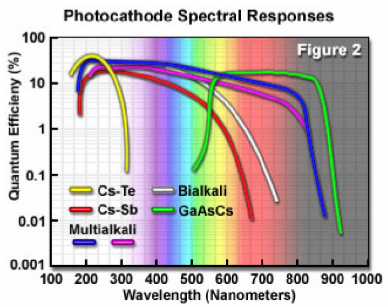
\includegraphics[width=0.7\textwidth]{immagini/efficienza_quantica.png}
\end{figure}
Vediamo come la quantum efficiency è fortemente dipendente dalla lunghezza d'onda, ad esempio ci sono fotocatodi che sono particolarmente ottimizzati per lavorare nel profondo UV e altri invece che lavorano a lunghezza d'onda più elevate. La scelta del fotocatodo dipende fortemente dallo scintillatore che adoperiamo e dallo spettro di emissione di questo, quindi bisogna cercare di far corrispondere queste due finestre di lavoro, cioè l'emissione dello scintillatore e l'assorbimento del fotocatodo.

\comment{

\subsection{Elettrodi di focalizzazione}
Una volta che sono stati emessi questi elettroni, dobbiamo cercare di convogliarli verso il primo dinodo
\begin{figure}[H]
   \centering
   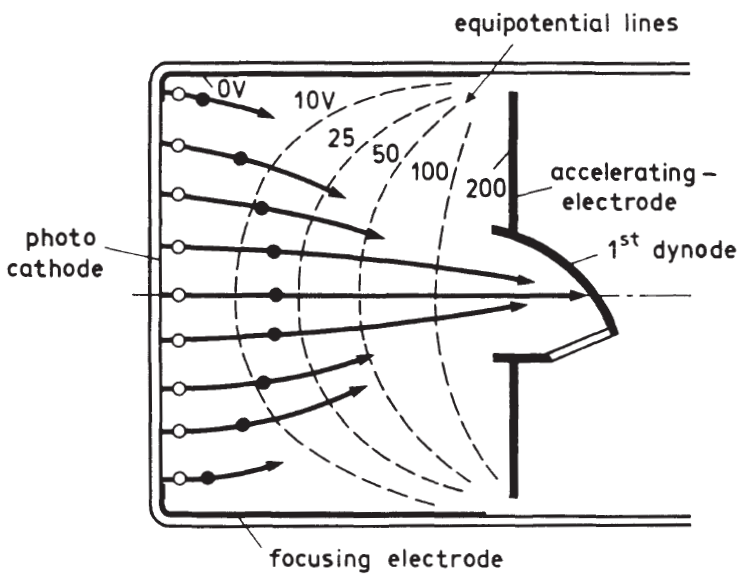
\includegraphics[width=0.7\textwidth]{immagini/elettrodo_di_focalizzazione.png}
\end{figure}
che in questa figura vedete è posizionato in questa zona questa è la finestra del fotocatodo queste sono le diverse diversi punti in cui può avvenire un'emissione perché chiaro che i fotoni ci dono su tutta la superficie del fotocatodo e quindi gli elettroni possono essere messi da diversi punti e pergiunte in diverse direzioni e con energia leggermente diverse che cosa vorremmo vorremmo che la raccolta sia una raccolta efficiente quindi tutti gli elettroni indipendentemente dalla loro energia indipendentemente dal punto in cui sono emessi vorremmo raggiungessero il primo dinodo ma per fare questo li dobbiamo in qualche modo guidare ecco perché questa prima regione presenta può presentare anche degli elettroni di focalizzazione quindi oltre ai dinodi si aggiungono degli elettroni ad esempio vedete qui sono mostrate degli elettroni di piani proprio per accelerare gli elettroni fargli seguire determinate determinati percorsi in base al punto in cui sono emessi e convogliarli verso il primo dinodo infatti allo di là di una questione di efficienza quindi di cercare comunque sia di convogliare tutti gli elettroni c'è un problema anche lo capiamo di timing perché capite che gli elettroni che benvano emessi nelle regioni più periferiche devono percorrere necessariamente un spazio maggiore per arrivare al primo dinodo e quindi rischierei di avere degli elettroni che arrivano dopo e questo comporta una indeterminazione dal punto di vista temporale che ovviamente qualcosa da evitare quando voglio adoperare uno scintillatore un fotomoltiplicatore per misure di timing con questo questo aspetto la profondiremo più là e quindi questa prima zona è una zona molto importante in un fotomoltiplicatore perché ci devono essere dei campi elettrici e addirittura alcune volte utilizzano anche dei campi magnetici proprio per ottimizzare focalizzare gli elettroni verso il primo dinodo a questo punto cerchiamo di capire cosa avviene nei vari dino di l'abbiamo già accennato prima ogni elettrone in grado di emettere ulteriori elettroni quindi elettroni vi diceva che vengono emessi con energia molto basse tipicamente dell'ordine dell'elettron volt e ogni dinodo è posto a un potenziale la differenza di potenziale di circa 100 volt rispetto a precedente in maniera tala al al che gli elettroni vengano guidati verso i dinodi successivi ora quando incide un elettrone lo vedete in questa in questa animazione che però è ve ve oscurata dalla barra sotto forse così lo vedete meglio vedete il tutto parte da un singolo elettrone l'elettrone incide sul dinodo e a quel punto può produrre ovviamente stato accelerato quindi acquisito una certa energia e a questo punto può estrarre dal primo dinodo un certo numero di elettroni e quanti ne estrae? Nel estrae all'incirca una trentina quindi ogni volta le incide un elettrone vemmeno emessi perfetti secondari una trentina di elettroni e questi elettroni devono essere accelerati verso il secondo dinodo ma in realtà non tutti questi elettroni riescono ad arrivare al secondo dinodo perché capite c'è anche qui un'efficienza di raccolta e di picamente solamente una frazione di questi elettroni arriva al secondo dinodo questa frazione mi porta a dire che all'incirca 5 elettroni su 30 riescono effettivamente ad arrivare al secondo dinodo quindi considerato questa efficienza il primo elettrone da era l'uogo in media a 5 elettroni che arrivano al secondo dinodo questo numero che io ho visto dicendo che normalmente intorno a 5 lo chiameremo delta ora vedremo che è importanza in termini di formazione del segnale quindi dovete immaginare che arrivano delta elettrone sul secondo dinodo e ogni uno di questi elettroni darà l'uogo nel terzo dinodo ad altri elettroni e così via allora c'è un ovviamente si evidenza un meccanismo di moltiplicazione lo vedete

anche da queste linee che diventano via via sempre più numerose ma manovesi passa da un dino al successivo quanto vale il fattore di guadagno cioè partendo da un solo elettrone alla fine su l'ultimo dinodo sull'anodo arriva un certo numero di elettroni quindi quanto vale il rapporto tra il numero di elettroni raccolte all'anodo rispetto al numero di elettroni prodotti dal catodo questo rapporto prende il nome di guadagno quindi mi dice sostanzialmente di quanto il fattore moltiplicativo di quanto ho guadagnato in termini di elettroni se parto da uno quanti ne ottengo alla fine e questo guadagno che in questo caso è indicato con G a volte trovate indicato con M dipende dal test consultate se vi fate il conto ogni volta appunto ogni elettrone amplifica di un fattore delta il numero di elettroni quando incide sul dino do questo guadagno sarà dato da questa formula alfa per delta inalzato a n dove n rappresente il numero di dino di questo numero dipende ovviamente da cambio la fotomoltiplicatore a fotomoltiplicatore però tipicamente potrebbe essere dell'ordine della decina che sopra per avere avere alfa invece è un fattore che assume grosso modo il valore uno e allora cerchiamo di capire quanto vale questo guadagno del fotomoltiplicatore se ad esempio abbiamo dieci dino di quindi dieci stadi di moltiplicazione alfa vale uno e delta vale cinque quindi da ogni elettrone incidente sul dino do se ne strabbero il cinque che riescono ad arrivare al secondo dino do allora le guadagno dato da questa formula e quindi vale a cinque inalzato a dieci cioè un valore di dieci alla sette quindi da un singolo elettrone nonostante le abbiamo persi parecchie perché abbiamo detto di 30 ne arrivano cinque quindi nonostante queste perdite riusciamo ad amplificare il numero di elettroni di un fattore dell'ordine di dieci milioni quindi tipicamente i fotomoltiplicatori hanno guadagni dell'ordine di dieci alla sei dieci alla sette sono numeri considerevoli quindi fa effettivamente il suo dovere anche se il segnale è molto debole riesce a produrre comunque sia un uscita un segnale in pensione abbastanza elevato grazie a questo fattore di moltiplicazione il fattore delta vi dicevo ha una sua importanza noi abbiamo fatto l'esempio di delta o la cinque ma in realtà è un valore medio capite che ogni volta di volta in volta questo numero di elettroni che viene messo che riesce ad arrivare al dino do successivo può cambiare su di scelere le fluttuazioni e queste fluttuazioni possiamo immaginare seguano la distribuzione di qua son ok quindi in media magari ne ho cinque però a volte capita che vedono emessi 4 elettroni che arrivano al dino do successivo oppure un numero maggiore sei sette chiaramente con una probabilità che può essere descritta dalla distribuzione di qua son e con una deviazione standard che se vi ricordate la distribuzione di qua son la possiamo immaginare come la radice di delta quindi se io dico che in media ne mettono emessi cinque in realtà sto dicendo cinque più o meno meno radice di cinque come deviazione standard e questo fattore delta ha un'importanza notevole quindi sulle fluttuazioni statistiche quindi il valore di delta è importante per capire anche cosa tendermi nelle fluttuazioni del segnale finale perché alla fine il segnale finale vi dicevo è dato da delta inalzato a n quindi una potenza di delta e quindi possiamo ragionare in termini di fluttuazioni statistiche sia ad esempio delta è uguale a cinque possiamo andare a guardare la distribuzione del numero di elettroni emessi dal primo dinodo allora questa distribuzione vedete cambia a seconda che si va a considerare appunto delta o alla cinque delta o alla quattro delta o alla tre chiaramente più è grande delta più queste fluttuazioni sembrano essere grandi cioè queste 

distribuzioni sono larghe ma in termini relativi effettivamente le fluttuazioni statistiche in termini relativi diminuiscono questo è appunto quello che avevamo detto anche nel caso della distribuzione di possono quindi se vengono emessi in meia cinque elettroni o ne vengono emessi venticinque quello che io mi aspetto è che le fluttuazioni statistiche in termini relativi chiaramente diminuiscono quando vado a considerare una emissione maggiore quindi un delta più grande e questo è una sua sua perché alla fine il segnale che si produce all'anodo tanto più elevato tanto più è probabile che si possa distinguere da un eventuale segnale di rumore perché immaginate ad esempio sul fotocatodo incidono dieci fotoni di questi maveri non li riveliamo tutti ne riveliamo una parte perché abbiamo quella quanto efficienzi di cui abbiamo discorso e quindi in uscita abbiamo un numero di foto elettroni che potrebbe essere due tre che danno luogo a un certo segnale a seguito di questo guadagno di cui abbiamo parlato questo segnale che si produce devo provare a distinguere da eventuali segnali di rumore tolvuto ad esempio e questioni termiche quindi che danno luogo a un segnale che tipicamente è molto frequente ma ha un'ampiezza piccola perché viene emesso un elettrone che da luogo a questa catena la giovitria ed edino di la disposizione è fondamentale perché vi dicevo questi elettroni devono essere guidati da un dino dall'altro e quindi in realtà ci sono tantissime configurazioni che sono state studiate nell'arco della storia in particolare quelle più utilizzate sono di quattro tipi che sono che che che messaggi relativi a zoom sono legati e sono quelli più utilizzati sono questi che vengono mostrati qui vedete a veneziana a box e a a focalizzati di niermento focalizzati circolarmente questi corrispondono a queste geometrie che vedete qui sulla destra non entraiamo nel dettaglio comunque quella che abbiamo visto fino adesso è quella di tipici quindi focalizzati linearmente che ha diversi diversi vantaggi ad esempio un aspetto che si può andare a cercare di capire in base alla configurazione scelta e sono le devienzioni dalla linearità quindi io mi aspetto che questo segnale vi dicevo mantengo una certa proporzionalità rispetto all'energia che viene depositata ma in realtà questo non è sempre vero a volte se il flusso di elettroni è molto elevato si può perdere la linearità quindi finché in questo grafico ad esempio la linea di devienzione della linea di sono pari a zero chiaramente stiamo lavorando in un ottimo regime di lavoro e questo ad esempio sono le curve che si ottengono per queste quattro configurazioni però non non non non non corrispondono questa abici di sono mi sbagliano corrispondono queste quindi ho riportato anche qui sotto la la descrizione del grafico che si legge appena perché l'abbiamo a barra davanti comunque sia quella migliore quella individuata dalla di corrisponde proprio a i i fotonottipicatori focalizzati linearmente infatti vedete che in una ampia regione di lavoro le devienzioni dalla linearità sono lo 0 per 100 ecco perché vi dicevo questa configurazione è una delle più adoverate effettivamente mentre le altre vedete riesco a mantenere le devienzioni della linearità dello 0 per 100 soltanto per basse correnti quindi basso numero di elettroni che viene prodotto e raccolta al lano do come avviene l'alimentazione vi dicevo banalmente si applica una un'alta tensione al tmt quindi voi il laboratorio ad esempio vi ritroverete all'applicare una tensione di 700 volt 700 volt ma in realtà poi questa tensione viene suddivisa tra i diversi dinodi andando a utilizzare dei partitori di tensione in generale vi dicevo c'è una particolare 

attenzione riguardo il primo dino do quindi ciò che viene tra il fotocato del primo dino do proprio perché il punto in cui noi dobbiamo andare a raccogliere in maniera più efficiente gli elettroni che vengono emessi dal fotocato do ci sono due modalità equivalenti di lavoro o si lavora con un fotocato a potenziale negativo e lano do a zero oppure viceversa il fotocato do zero e lano do ha una tensione positiva sono due modi diversi di lavorare ma alla fine l'importante è la differenza di potenziale che si deve passare da un potenziale più basso un potenziale più alta alla fine andiamo a guardare un altro aspetto quindi questa tensione di alimentazione del fotomoltiplicatore che influenza a sul segnale finale questo fattore delta che vi dicevo in realtà io vi ho ho è grosso modo 5 ma può cambiare a seconda della tensione di lavoro più e alta la tensione di lavoro più gli elettroni verranno accelerati tra un dino dell'altro quindi raggiungeranno energie più alte maggiore sarà il numero di elettroni emessi quindi di elettroni che riescono ad aggiungere al dino do successivo quindi questo fattore delta cambia a seconda della tensione di alimentazione allora se immaginiamo di indicare con vi condì la differenza di potenziale tra due dino di consecutivi delta è dato da k per vi condì dove k è una costante di proporzionalità e vi condì questa tensione e allora il guadagno che l'avevamo espresso come alpha per delta inalzato a n si può andare a riscrivere in termini di tensione alpha per k v inalzato a n dove n è il numero di dino di quindi abbiamo una legge di potenza il guadagno dipende dalla tensione non in modo lineare ma attraverso una legge di potenza v inalzato a n Quindi basta anche una leggera variazione nella tensione di lavoro per avere una variazione nel guadagno notevole proprio a causa di questa potenza all'N. Ecco perché gli alimentatori che si adoperano per alimentare i fotomoltiplicatori devono essere degli alimentatori abbastanza stabili, quindi che mantengono il valore di tensione il più stabile possibile. Ma possiamo essere interessati a cercare di capire quanto varia il guadagno quando variamo la tensione di un volt. E allora questa variazione che normalmente si esprima in termini percentuali prende il nome di coefficiente di guadagno ed è qualcosa che andrete a misurare il laboratorio. Infatti misurare il guadagno del fotomoltiplicatore non è un'operazione facile perché per misurare il guadagno voi dovreste lavorare in condizioni di singolo fotoelettrone, quindi mettervi nelle condizioni di far produrre un fotocato di un sole elettrone e vedere cosa si ottiene all'anodo. E questo non è qualcosa di semplice, dovete avere un sistema calibrato, quindi la misura del guadagno non è banale. Però si può studiare l'andamento del guadagno in funzione della tensione e quindi valutare queste variazioni percentuali del

guadagno al vadeare della tensione. Vedete quello che farete il laboratorio, quindi proverete ad acquisire, ad effettuare delle misure con un fotomoltiplicatore, aumentando di volte in volta la tensione, esplorando un certo intervallo di tensioni e andando a cercare di capire quanto cambia il vostro segnale in uscita. Il segnale cambierà ovviamente la sua ampiezza perché aumentando la tensione aumenta il guadagno, quindi aumenta il numero di elettroni che arriva all'anodo e il vostro segnale aumenterà in ampiezza. Quindi voi possiamo studiare di quanto aumenta o diminuisce il vostro segnale quando cambiate la tensione di un certo valore. E quindi possiamo studiare la derivata dell'ampiezza del segnale in funzione della tensione, ritrovare una legge di potenza di questo tipo e valutare il coefficiente di guadagno, che è qualcosa che vincevo, dovete fare in laboratorio e lo farete appunto in questo primo turno di esperienza. Chiaramente il coefficiente di guadagno viene espresso in percentuale su volt. Andiamo a guardare un altro aspetto del fotomultrificatore e cioè la risposta temporale. Allora tipicamente gli elettroni vengono emessi con tempi molto rapidi, un decimo dinano secondo, grossomodo. Tuttavia la cosa che conta di più nella produzione del segnale in termini temporali è il tempo che impiegano questi elettroni per passare dal catodo fino all'anodo. E questo è un tempo che non è trascurabile ed è l'ordine delle decine di l'anno secondi. Quindi per percorrere tutto quel percorso tra i dinodi è necessario un intervallo temporale di circa dieci nanosecondi. Forra se questo tempo fosse fisso, fosse costante, fosse sempre lo stesso ogni volta che viene messo un elettrone dal catodo non avrei alcun problema. Nel senso sarebbe un ritardo noto, non lo fornisce il costruttore quindi so quando effetto una misura di timing che è presente questo ritardo. Quindi da quando incide la radiazione e quando viene rivelata mi aspetto un ritardo fisso. Il problema in realtà è che per diverse ragioni esiste una indeterminazione, una dispersione di questo transit time, di questo tempo di transito che prende il nome di tts transit time spread. Quindi è vero che magari il tempo medio per percorrere il fotomoltiplicatore dell'ordine della decina di nanosecondi però rispetto a questo tempo medio o delle fruttuazioni che possono essere anche dell'ordine di alcuni nanosecondi. E questo chiaramente limita l'utilizzo del fotomoltiplicatore per applicazioni di timing, spinto ovviamente, dove magari voglio risoluzioni temporali particolarmente ottimali dell'ordine e comunque inferiori a nanosecondo. Come si può migliorare questo aspetto? Allora ci sono dei fotomoltiplicatori che magari migliorano questo aspetto con un'opportuna geometria del dinodino di oppure diminuendo il numero di fotoelettroni, quindi lavorando in condizione di illuminazione del fotomoltiplicatore un po' più basse però non sempre è possibile. Un ultimo aspetto che volevo discutere sui fotomoltiplicatori riguarda il fatto che i fotomoltiplicatori devono lavorare lavorando con elettroni di pochi elettron volte l'abbiamo detto e quindi sono elettroni molto poco energetici che possono subire delle deviazioni anche a seguito della presenza del campo magnetico terrestre. Ecco perché i fotomoltiplicatori a seconda di come vengono orientati, in lì e di principio potrebbero funzionare in maniera vengermente diversa perché potrebbero avere un orientamento rispetto al campo magnetico terrestre diverso secondo di come viene posizionato il fotomoltiplicatore. Per evitare questi aspetti, questi problemi, quello che si fa è circondare il fototubo con un materiale che si è in grado di schermare questi campi magnetici non eccessivamente elevati come ad esempio il campo magnetico terrestre e questi

materiali è tipicamente prendere il nome di MuMetal che sono delle levi e metalliche adalta per miabilità magnetica quindi formano un vero e proprio schermo per i campi magnetici, maniera tale che gli elettroni che vengono prodotti all'interno non surviscono effetti di deviazione dovute a questi campi magnetici così poco intensi. Tuttavia capite che certe volte si ha l'esigenza di posizionare i fotomoltiplicatori all'interno dei campi magnetici di valore più elevato perché magari in fisica si vuole provare a misurare l'impulso di una particella deviando il percorso della particella con campi magnetici che possono essere anche molto più intensi rispetto a quelli tipicamente derivanti da fonti naturali. Allora in questo caso i fotomoltiplicatori non possono essere adoperati, ve l'avevo detto anche prima nel caso della PET. Quello che si fa è eventualmente trovare dei degni sostituti del fotomoltiplicatore che ora andremo a vedere e che possono lavorare anche in presenza di campi magnetici. Un aspetto importante riguarda il rumore, il noise già l'avamo visto, la principale fonte di rumore in un fotomoltiplicatore è l'emissione termodionica di elettroni da parte del fotocato, ma anche da parte di altri materiali che costituiscono il fotomoltiplicatore. Tipicamente vi dicevo viene messo un solo foto elettrona alla volta, ecco perché il segnale che si produce un segnale spurio, cioè dovuta rumore, in questo caso un segnale di bassa ampiezza ed è importante quindi avere i segnali fisici invece più elevati in maniera tale da poterli discriminare dal rumore. Può essere diminuito, vi dicevo, abbassando la temperatura, ma questo non lo so, si fa quasi mai. Inoltre un altro aspetto importante sempre in termini di rumore è quello di evitare di esporre il fotomoltiplicatore alla luce anche quando non si sta lavorando col fotomoltiplicatore, quindi immaginate di prendere un fotomoltiplicatore e trasportarlo da una stanza nell'altra dovete avere la cura, la cortezza di evitare l'esposizione alla luce, questo perché i materiali vetrosi che avevano adoperato soprattutto nel cato do, possono emettere luce di fosforescenza anche per tempi molto lunghi, anche nelle ore successive, quindi se per caso il fotomoltiplicatore viene sforza alla luce poi bisogna attendere un tempo che può essere anche dell'ordine delle ore prima di poterlo adoperare, altrimenti potremmo avere effetti indesiderati dovuti proprio questi fenomeni di fosforescenza del vetro. Oltre a questo aspetto poi ci sono altre fonti di rumore in un fotomoltiplicatore che possono essere derivanti ad esempio dalla radiatività del vetro, infatti nel vetro possono essere presenti degli i sottopi radiativi come il potassio 40, al torio che emettono ovviamente radiazione che viene amplificata nel fotomoltiplicatore, radiazione cosmica che incide non solo sul rivelatore ma anche all'interno del tubo oppure ci potrebbero essere correnti di fuga nei supporti degli elettro di 11C, ci vuolano particolare cura nel cercare di isolare gli elettro di presenti in un fotomoltiplicatore. Un altro aspetto che potrebbe verificarsi sono i cosiddetti after pulses, guardate ad esempio questo è un tipico segnale da un fotomoltiplicatore come viene visto in uno oscilloscopio quindi ovviamente quello che si rappresente qui è un asse temporale e l'asse su cui si visualizza il segnale prodotto all'anodo, vedete un segnale molto veloce, la scala non ci aiuta però veramente il tempo di discesse molto rapido dall'ordine del nano secondo, pochi nanosecondi, il segnale risale e dopo che è risalito vedete qui la presenza di piccoli impulsi di bassa ampiezza, questi prendono le nome di after pulses, sono degli impulsi che avvengono dopo il segnale principale e possono avere delle conseguenze importanti soprattutto nelle misure di timing perché le misure di timing ovviamente prevedono un start, uno stop quindi se per caso ci sono degli impulsi spuri lo start e lo stop potrebbero non essere quelli effettivamente desiderati. Le fonti di questi after pulses che sono sempre delle 

ovviamente fonti di rumore per noi possono avere diverse origini o delle reazioni luminose cioè i dino di colpiti dagli elettroni possono emettere dei fotoni che se arrivano al fotocatodo, quindi tornano indietro verso il fotocatodo, possono dare origine ad un effetto fotoelettrico e quindi produrre questi after pulses che sono ovviamente ritardati rispetto all'impusso principale perché dobbiamo considerare il tempo che impiega la luce attorno indietro verso il fotocatodo e i ritardi tipici in questo caso sono dell'ordina di 20, 100 nanosecondi, oppure ionizzazione del gas residui nel fototubo, non ve lo ho detto ma il fototubo, questo tubo che abbiamo visto dove sono inseriti i dino di ovviamente lavora in condizioni di vuoto possiamo dire, però per quanto possa essere spinto il vuoto realizzato all'interno del fototubo sempre sono presenti delle molecole, degli atomi di gas residuo e quello che può succedere è che gli elettroni possono ionizzare questo gas residuo e gli ioni positivi possono migrare verso il fotocatodo perché ovviamente il fotocatodo si trova a un potenziale negativo e liberare elettroni e quindi produrre dei segnali ritardati con ritardi tipici di 100 nanosecondi o anche microsecondi perché dovete immaginare che questo impulso viene prodotto da un ione che ha dovuto viaggiare verso il fotocatodo e quindi ovviamente con una mobilità ridotta oppure potremmo avere effetti di backscattering degli elettroni e quindi durante il processo di amplificazione alcuni di questi elettroni che avevano messi i retino di anziché viaggiare verso il vino del successivo tornano indietro generando un altro segnale ritardato quindi queste sono tutte possibili fonti di after falses che purtroppo sono sempre presenti in un foto moltiplicatore vi dicevo le dimensioni della forma possono essere anche qui molto su variate tipicamente sono oggetti ingombranti in ogni caso hanno normalmente questa forma tubolare a forma di cilindro questo è un tipico fotomoltiplicatore vedete qui la finestra di ingresso il fotocatodo appare proprio come un vetro ma potrebbe avere anche forme un po più particolare ad esempio questo un fotomoltiplicatore di grande area perché sono fotomoltiplicatori che venono ad esempio adoperati nell'esperimento km3 net l'esperimento per la rivelazione dei neutrini che stanno installando il capo passero in quel caso il motivo di utilizzare un fotomoltiplicatore di dimensioni così grandi consiste nel cercare di andare a accattare un quantitativo di luce che sia il più grande possibile perché già di persa la luce prodotta in mare dall'interazione dei neutrini quindi dei muoni è abbastanza bassa quindi bisogna raccogliere il più possibile la luce prodotta vi dicevo ci sono tantissime applicazioni dei fotomoltiplicatori non solo nel campo della della fisica ma anche in medicina e biologia ad esempio una delle applicazioni più note di fotomoltiplicatori nel campo della fisica riguarda l'esperimento supercambio cande non so se ne abbiamo parlato non abbiamo parlato non abbiamo affrontato ancora neutrini niente non abbiamo parlato di neutrini va bene comunque questo è un grosso rivelatore che è stato realizzato all'interno di una miniera abbandonata questa miniera è stata riempita di acqua e le panetti sono state ricoperte vedete da questi fotomoltiplicatori di grande area e il motivo appunto che i neutrini interagendo con l'acqua possono produrre ad esempio muoni che poi emettono ovviamente della radiazione nell'attraversare l'acqua per pareffetto cerenco quindi massiva misurare questa radiazione vedete sono tanti occhi insostanzialmente questo esperimento ha lavorato per diversi anni vedete qui ad esempio una fase di intervento queste sono delle persone su un buon muone che vanno a sostituire comunque a intervenire su alcuni di questi 

fotomoltiplicatori questo esperimento diceva ha preso dati per tantissimi anni diversi anni fa c'è fu un incidente si rupperò praticamente tutti i fotomoltiplicatori attraverso una reazione a cadena cioè si si si è rotto un fotomoltiplicatore e poi sono esposito tutti gli altri comunque ormai mi sembra che non prenda più dati questo estremento oppure ad esempio nel campo del raggi cosmici raggi cosmici nell'attraversare l'attraversfera possono produrre luce di florescenza anche questa è una luce molto debole e utilizzando degli opportuni telescopi di florescenza si può convogliare attraverso un sistema di specchi la luce di florescenza verso un fotosensore che in questo caso è costituito da fotomoltiplicatori ad esempio l'esperimento ger che è il più grande esperimento per la fisica dei raggi cosmici utilizza proprio sistemi di questo tipo oppure al ser non ovviamente ci sono tantissimi rivelatori che utilizzano questo tipo di fotosensori ovviamente e qui il problema è al solito l'utilizzo di campi magnetici e in questa tabella vedete giusto per avermi idea i diversi esperimenti che fanno uso di scintillatori e di fotomoltiplicatori ovviamente sono anche grossi numeri quelli in gioco anche nel campo della ricerca dell'antimateria sulla soluzione spaziale sono installati i rivelatori come ad esempio ams che presenta il termine dei fotomoltiplicatori quindi gli impieghi sono veramente molto ampi anche nel campo della bioluminescenza quindi la rivelazione di luce messi ad organismi viventi anche questo caso siccome la luce messi è molto debole si utilizzano dei fotomoltiplicatori tuttavia i fotomoltiplicatori hanno delle problematiche l'abbiamo detto e anzitutto a volte hanno delle dimensioni troppo grandi rispetto all'area sensibile sono influenzati dai campi magnetici hanno una risposta spettrale che non sempre è adatta alla luce da rivelare una efficienza quantica che abbiamo visto non è città l'ordine di 20 30 per cento la stabilità del guadagno quindi quanto è stabile questo guadagno che abbiamo definito insomma non è ottimale dipende molto dalla tensione inoltre dobbiamo doverare delle tensioni di alimentazione elevate diverse centinaia di volte fino anche al chilo volte quindi ci sono diversi aspetti negativi è proprio per questo motivo nel corso degli anni sono stati sviluppati dei fotossensori più recenti più compatti basati sull'utilizzo di materiale semiconduttore quindi si sono dei fotossensori ha stato solido in particolare oggi vedremo e li avranno scoperto da io si si dicono i propri players i primi prototipi di app di sono stati sviluppati ormai una quarantina d'anni fa inizialmente i primi prototipi avevano dimensioni molto piccole superfici dell'ordine del millimetro quadro inoltre erano particolarmente sensibili all'infrarosso quindi magari non si adattavano quelli scintillatori che mettevano nell'ov avevano un basso guadagno che costa molto davvero sembravano dei rivelatori non particolarmente performanti ma in anni recenti ovviamente sono state migliorate diverse caratteristiche di questi fotossensori quindi adesso abbiamo degli app di che hanno superfici più estese dell'ordine di decine dei millimetri quadri quindi tre per tre millimetri quattro per quattro millimetri insomma sono già dei sensori non superfici più grandi hanno una sensibilità maggiore già nel blu e l'ultravioletto che è quella che ci interessa di più soprattutto per la luce di scintillazione il costo si è abbassato e hanno una guadagno relativamente elevato vi dico relativamente perché comunque sia confrontato con il guadagno del fotomultilitatore che abbiamo detto dell'ordine di 10 alla 6 10 alla 7 qui proprio per il principio di funzionamento dell'app di non si superano guadagni di 100 lo secondo quindi stiamo parlando della decina come il guadagno e hanno l'enorme vantaggio di lavorare con tensioni più massi rispetto a quella dei fotomultilitatori. Venono utilizzati proprio per questo motivo in diverse applicazioni dove sono presenti gli scintillatori. Qual è il principio di funzionamento vedremo un po più nel dettaglio i riferatori sono solido quando parleremo proprio di questa categoria di riferatori per adesso spero che appunto abbiate 

perché conoscenze di base, di fisica, dei semi-conduttori comunque quello che si fa è ad operare dei materiali semi-conduttori però non pure ma drogati, cioè vuol dire che alcuni atomi sono stati introdotti alcuni atomi di un elemento diverso che possono essere elementi donori quindi con un eccesso di elettroni rispetto a un atomo che costituisce voyage cristallo oppure accettori e quindi tipicamente voi troverete materiali drogati di tipo P o di tipo E. Secondo del tipo di elemento che abbiamo utilizzato per drogare i semi-conduttori. Alla no realizzare delle particolari unzioni è possibile creare dei rivelatori con i seguimi conduttori, i rivelatori di particelle non vedremo, ma anche rivelatori di luce. Quindi tipicamente una PD ha una struttura come quella che vedete qui schematizzata, quindi vedete una sequenza di materiali dove abbiamo una parte intrinsega, dove avere intrinsegolo, vuol dire un materiale che non è stato drogato, ma vuol dire un materiale che è stato drogato con la stessa concentrazione di atomi, donori e accentori. Poi abbiamo, vedete, un primostrato drogato di TPP, poi abbiamo un altrostrato drogato di TPP e di TQN. Insomma abbiamo una sequenza di strati dove si viene a realizzare una regione ottimale per la rivelazione, quindi se guardate qui schematicamente la stessa struttura sostanzialmente, quando incide un fotone con energia HN viene prodotta in questa regione, quella regione di rivelazione, una poppia elettrona in lacuna e grazie all'utilizzo di elettro, di vedete qui viene creato una differenza di potenziale tranne o decatodo, questa elettrona emigra, ovviamente viene accelerato e può produrre soprattutto in questa regione P ed N più dei processi di moltiplicazione a valanga, ecco perché avalanci fotondaioz, nuovamente un po' come avveniva per in gas, se vi ricordate, anche qui l'elettrone può arrivare ad avere un'energia sufficiente a estrarre e produrre nuove poppie elettrone lacuna, con ovviamente un guadagno anche in questo caso che vi dicevo non supera il valore di 100, quindi possiamo da un fotone incidente quindi un elettrone prodotto al massimo ottenere un centinaio di elettroni raccolti nel nostro elettro d'ofinale, quindi capito i segnali non menvano amplificati di molto, ma quel che serve per la rivelazione di questi fotoni. Andiamo a guardare alcune caratteristiche di questo APD, allora in azitudine abbiamo un strato anti riflesso in superficie e quindi grazie a questo abbiamo un'elevata efficienza di rivelazione perché la maggior parte dei fotoni coincide riesce effettivamente a essere rivelata. La tensione di alimentazione vi dicevo è più bassa dell'ordine di alcune centinaia di volt, però i guadagni non sono elevatissime, 50-100, grosso modo. Anno inoltre 

come tutti i rivelatori e semiconduttore è purtroppo una dipendenza dalla temperatura, quindi variare la temperatura di lavoro chiaramente comporta delle variazioni nel segnale in uscita, possiamo avere anche qualche per cento di variazione per ogni grado di temperatura, quindi lavorare una temperatura statabile è importante, ma in generale vale per tutti i rivelatori e casse e decomittore. Sono particolarmente adatti per convertire la luce proveniente da Fibre, Wevel e Shifter perché le Fibre, Wevel e Shifter hanno dimensioni piccole, hanno sezioni piccole quindi andare ad accoppiare un rivelatore piccolo è utile in questo caso, o a partire da piccoli scintillatori, chiaro che uno scintillatore di dimensioni grandi non può essere accoppiato come un superficie sufficiente ad assicurare la rivelazione dei fotoni di scintillazione, hanno delle proprietà temporali di timing abbastanza buone e vi dicevo ormai le dimensioni possono arrivare anche a 5 per 5 mm quadri, vedete qui un esempio di APD dove la parte sensibile è questa parte in nero. Il segnale è proporzionale al numero di fotoni incidenti, quindi manteniamo l'informazione sull'energia depositata o comunque sullo numero di fotoni incidenti e vedete qui ad esempio con un APD di questo tipo, giusto per capire le dimensioni, qui abbiamo una monetina non so se un centesimo o docentesimo con una monetina in rame e vedete le dimensioni dei fotodiodi e qui abbiamo un piccolo cristallo come quelli che avevano operato ad esempio per l'aperta che hanno dimensioni veramente piccole, a questo punto potrebbero essere detti tranquillamente con un APD. Una applicazione che abbiamo fatto all'interno dell'esperimento lì dice di cui ci siamo occupati, riguardavo l'utilizzo di fotoni, per andare a leggere da luce raccolta da fibre wavelength shifter, vedete le fibre che vi ho portato una volta scorsa sono esattamente queste e queste fibre corrono all'interno di un modulo che è costituito da strate alternati di piombo e scintillatore che veniva doperato proprio per un calorimetro, in questo caso quindi la luce prodotta nello scintillatore veniva raccolta da queste fibre e le fibre venivano confondinate sulla superficie dell'APD, quindi vedete ci sono diverse applicazioni anche se la superficie non è particolarmente estesa ci possono essere delle soluzioni che permettono di doperare l'APD anche con rivelatori di dimensioni più grandi e qui era fondamentale perché chiaramente si alimenta luce e lavora all'interno di un campo magnetico quindi un fotomultivitore si sarebbe prodotto in caso per l'area. Concludiamo andando a guardare l'ultima categoria di rivelatori un po più recenti di fotosensori in silicon photomultipliers quindi capite il fatto che si adoveri la parola fotomoltiplicatore vi fa capire che evidentemente qui di guadagno è più elevato più simile a un fotomultivitore quindi abbiamo il vantaggio di avere un guadagno elevato ma abbiamo un materiale semiconductor infatti anche in questo caso abbiamo l'utilizzo di un rivelatore che è molto simile all'APD dovete immaginare che un sito è costituito da una matrice di APD di piccolissime dimensioni quindi come se fosse un rivelatore a pixel, un ipixel è una sorta di APD. Ora come funziona? Tutte queste cele che vedete che possono avere diciamo delle dimensioni dalle decine, le centinaia di micron quindi abbiamo densità molto elevate dell'ordine di 1000 pixel per millimetro quadro tutte queste cele lavorano in parallelo quindi se il vione di queste cele viene colpita da un fotone e quindi dal luogo a un segnale io posso andare a sommare tutti questi segnali tra di loro e quindi avere un segnale l'uscita che è proporzionale a quante cele sono state colpite dai fotoni e quindi è proporzionale a quanti fotoni hanno inciso sul rivelatore. Chiaramente tutto questo discorso ha una sua validità finché parte del presupposto che su ogni singola celle incide un solo fotone è chiaro. Se dovessero incidere più fotoni perdo ovviamente questa linearità che è il supposto però normalmente i sito siccome hanno celle di 

dimensioni molto piccole normalmente lavorano in queste condizioni di linearità quindi vedete qui uno schema di questi di questi sito ma dove possiamo vedere le diverse cele ognuna di queste cele ha una sua resistenza di spegnimento di quenching per poter riportare la celle poi con una certa costante caratteristica verso le condizioni di lavoro ottimali e quindi sostanzialmente la vorra come se fosse un rivelatore multiplo quindi tanti rivelatori che lavorano insieme ma alla fine prelevo un solo segnale che è la summa dei segnali di tutte le celle. Con i vantaggi A in anzi tutto lavorare attenzioni molto basse, inferiori a 100 volt, ha un'efficienza quantica che questi sono numeri un po' vecchiotti ma già siamo arrivati anche ai 50\% quindi è abbastanza elevata. Hanno due danie elevati 10 alla 6 proprio perché a questo punto il tutto dipende da quanti pixel abbiamo l'esposizione. La risoluzione temporale è molto buona, sono indipendenti dal campo magnetico, tuttavia ancora si deve lavorare un po' sulle dimensioni e sul dark count rate quindi quel rumore che è sempre presente nei dispositivi, nei fotosensori, anche in essenza di radiazione che in questo caso può essere anche molto elevato, dipende dal produttore ma anche in questo campo ci sono stati dei notevoli sviluppi ormai si arriva anche a un kilo eazzo per milimetro quadro che è qualcosa di molto soddisfacente. Vediamo alcuni esempi, ci sono diverse ditte che producono questi dispositivi, l'esempio la più famosa è una ditta giapponese che prende il nome di Amamatsu e vede appunto questi piccoli dispositivi. Vi dicevo le celle lavorano in parallelo e quindi se andiamo a guardare all'oscilloscopio un tipico segnale prodotto da un silicon photomultiplier questi segnali se li mettete in persistenza, cioè non fate aggiornare i display dell'oscilloscopio ma ad accumulare tutti i segnali che vi arrivano nel tempo, quindi non si cancella, quello che è stato visualizzato prima ma mi rimane nello schermo e non segnale viene sovrapposto a quello che abbiamo visto prima. Quello che osserverete se abbiamo un buon SIPM è una distribuzione dei segnali come quello che vedete qui, che cosa stiamo vedendo? Stiamo vedendo dei segnali che non hanno ampiezza qualunque, hanno ampiezze quantizzate quindi assumono dei valori tipo discreti o ad esempio in corrispondenza di questo livello o in corrispondenza del doppio, del triplo, che cosa stiamo vedendo? Stiamo vedendo la rivelazione dei singoli fotoelettroni, quindi avendo un segnale ad esempio che è questa ampiezza equivale ad aver misurato un solo fotoelettrone, quindi è inciso un solo fotole che ha dato l'uovo a una sola scella colpita. Se ne avevano colpite due abbiamo un segnale che ha una ampiezza doppia, se ne vengono colpite tre vedete il triplo e così via, quindi si vede questa discretizzazione, questa quantizzazione, perché ogni cella lavora come se fosse un guide, quindi un rivelatore on off. Ok, un attimo metto a caricare il computer prima che si scarica, vediamo un po' la situazione della batteria, no, beccia, dovrei fare. Se andate a realizzare uno spettro delle ampiezze di questi segnali, chiaramente troverete una distribuzione a picchi, lo faccio vedere meglio, perché corrisponde al fatto che le ampiezze non sono quelle, ma assumono dei valori ben precisi, quindi ad esempio questo primo picco è quello corrispondente al primo fotoelettrone, il secondo picco è quello corrispondente al due fotoelettrone, così via. Guardiamo l'ultimo aspetto, anche qui abbiamo una efficienza di rivelazione, una photo detection efficient, che però dipende da diversi parametri, abbiamo un aspetto derivante dal film factor per vedere cos'è, l'efficienza che abbiamo visto per le foto cattle di un colore che dipende della condizionata, che è una propapriità di trigger della valore. In particolare il film factor dipende dal fatto che abbiamo una matrice e quindi l'area sensibile ovviamente la parte centrale, ma abbiamo inevitabilmente dei bordi che rappresentano un'area morta, quindi se il fotone dovesse incidere su questi bordi, non riverrebbe perso, quindi questo è un contributo, ovviamente il rapporto tra l'area effettivamente attiva di rivelazione e l'area complessiva, quindi più siamo in grado di realizzare i sottili, maggiore sarà l'efficienza dovuta al film factor. Capite che l'effetto del borbe è tanto più importante quanto più è piccola la dimensione del pixel, quando il pixel è più grande il borbe ha un effetto minore. Comunque normalmente possiamo avere

anche film factor che variano dal 30\% fino all'80\%, dipende chiaramente dallo dispositivo. L'efficienza quantica è più elevata rispetto a quella che abbiamo visto nel caso dei fotomoltiplicatori tradizionali, vedete può assumere valori anche superiori all'80\%, dipende ovviamente dal tipo di sensore e dalla longhezza donna che andiamo a rivelare. Infine abbiamo anche una probabilità di trigger, una volta che ha inciso la radiazione e ha prodotto una poppia riesce a produrre questa poi un segnale sufficientemente elevato, quindi a dare luogo a un trigger, quindi a una rivelazione e questo dipende sostanzialmente dalla tensione. Vedete quei due curve che variano con il campo elettrico applicato, quindi con la tensione e che ciò a vedere appunto che la probabilità di trigger cresce ovviamente con la tensione applicata. Per i SITM ci sono diverse strutture anche qui vediamo diversi strati di materiale del drogato e tipicamente si distinguono in P2N o N su PES, quando di quale la regione è sensibile, se è una regione di TPUN o una regione di coppia, comunque questi sono dettagli più postruttivi. Possono essere adoperati siccome hanno dimensioni molto piccole un po come il caso degli APD per la lettura delle fibre VLS, soprattutto quando abbiamo mandato una sola fibra quindi vi è aspettata poco a luce, il SITM avendo un guadagno notevole è un ottimo candidato per la rivelazione di questa luce. Infatti vedete qui ad esempio degli scintillatori dove sono stati realizzati dei solchi dove è stata messa la fibra VLS ai capi della fibra si va a posizionare un SITM, quindi ci sono tantissime applicazioni di questo tipo. Anche per la PET si sta pensando sostituire il classico cotocontribilitatore con dei silicon photomotivlier, sono degli ottimi candidati quindi riassumendo, confrontando questi fotosensori da un lato abbiamo il PMT che si caratterizza per avere degli ottimi guadagni ma ha una tensione di lavoro molto elevata con un dark count rate abbastanza basso, altro difetto e efficienza quantica bassa ma la selleraria sensibile è abbastanza elevata. Poi abbiamo i materiali semi-conduttori quindi APD e SITM che si caratterizzano soprattutto dalle basse tensioni di lavoro hanno però come svantaggio il fatto di avere delle superfici abbastanza ridotte ma hanno efficienze tipicamente più elevate, con guadagni che possono anche essere confrontabili con quelli del fotomotivlidatore tradizionale. Devo attaccare il carica batteria prima che si scolle da tutto. Anche lo srotchio in realtà lo possiamo immaginare come un fotosensore, non so se conoscete la struttura interna dell'occhio, sapete che appunto la luce alla fine dopo aver attraversato diversi strati di materiale diverso. Arriva a incidere sulla retina, la retina dovete immaginare come se fosse un vero e proprio rivelatore anche se costituita da una sorta di pixel che sono i nostri fotorecettori. Infatti la retina è costituita da coni e basso in celli, secondo se siete interessati alla visione di urna, dei colori o alla versione notturna crepuscolare. Intervengono dei recettori, fotorecettori diversi, in particolare i coni sono destinati alla visione di urna, quindi la percezione dei colori sono un numero più ridotto rispetto ai basso in celli, tipicamente si concentrano vicino nella parte centrale della retina, vicino all'asse ottico. I basso in celli invece che sono utilizzati per la visione notturna sono molti di più e sono distribuiti un po' in tutta la regione della retina. Comunque perché faccio questo discorso? Perché potremmo cercare di capire che prestazioni ha il nostro occhio in termini di auto rivelazione. Alla fine noi abbiamo parlato di strumenti che vanno a percepire della luce che il nostro occhio è lì in principio e non è in grado di percepire, o comunque non è facile percepirli. Allora in totale posso immaginare di avere un occhio standard all'incirca 100 milioni di fotorecettori, quindi equivale al dire 100 megapixel se dovessimo adoperare un termine simile a quello che doveriamo nel campo della rivelazione e in una singola immagine vengono interessati simultaneamente all'incirca 7 megapixel. Tuttavia l'occhio vede continuamente in modo ciclico anche 100 volte al secondo e questo ne aumenta la risoluzione. Quindi alla fine potremmo dire che complessivamente il nostro occhio può essere approssimo all'autofotosensore con 570 megapixel, quindi immaginate ovviamente delle prestazioni notevoli. Chiaramente la sua risposta dipenderà dalla lunghezza d'onda della luce che incide, in particolare di nostro occhio ottimizzato per vedere le lunghezze d'onda intorno al verde e giallo che appunto corrispondono anche col massimo di emissione della nostra stella nel sole, quindi non è un caso ovviamente che noi abbiamo una maggiore risposta proprio in corrispondenza di queste lunghezze d'onda. Concludo facendovi vedere questo articolo che uscito qualche anno fa a Sonnecer, è stato appunto una notizia particolare, io insegnavo a Topp, fin l'anno scorso e quindi mi interessavo anche di questi aspetti, sostanzialmente è stato condotto uno studio per cercare di capire se l'occhio umano fosse in grado di rivelare di riperrare i singoli fotoni, cosa che noi normalmente facciamo appunto con della strumentazione anche molto costoso e complessa, ma in realtà è stato dimostrato sperimentalmente che l'occhio umano è in grado di misurare i singoli fotoni, è stato fatto appunto uno studio sperimentale sotto determinate condizioni e si è arrivato questo risultato che ha meritato la pubblicazione su Nexar, non so se conoscete vostre riviste, penso di sì, quindi sapete che non è rivista di assoluto prestigio e questo è contestato il riassunto di questo risultato sperimentale.
}